\documentclass[tikz]{standalone}
\usepackage{tikz}
\usetikzlibrary{calc}

\newcommand{\functionBox}[7]{%
  \begin{scope}[shift={(#1, #2)}]%
    \def\boxwidth{#3}
    \def\titleheight{#4}
    \def\bodyheight{#5}

    \draw[thick] (0, 0) rectangle (\boxwidth, -\titleheight - \bodyheight);
    \draw (0, -\titleheight) -- (\boxwidth, -\titleheight);

    \node[anchor=mid, align=center]
      at (\boxwidth/2, -\titleheight/2)
      {\textbf{#6}};

    \node[anchor=north west, align=left, font=\footnotesize]
      at (0.1, -\titleheight - 0.1)
      {#7};
  \end{scope}%
}

\begin{document}
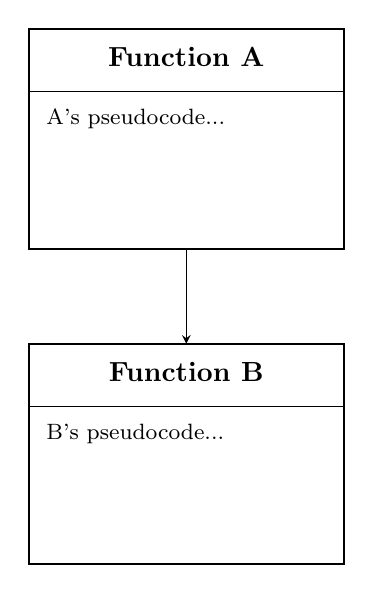
\begin{tikzpicture}[>=stealth]
  % Create boxes using \functionBox
  \functionBox{0}{0}{4.0}{0.8}{2.0}{Function A}{A's pseudocode...}
  \functionBox{0}{-4}{4.0}{0.8}{2.0}{Function B}{B's pseudocode...}

  % Create named boxes using \functionBoxNamed
  %\functionBoxNamed{A}{0}{-5}{Function A}{A pseudocode}
  %\functionBoxNamed{B}{0}{-9}{Function B}{B pseudocode}

  % Connect them using named anchors
  \draw[->] (2, -2.8) -- (2, -4);
\end{tikzpicture}
\end{document}

